\chapter{Implémentation}
\label{ch:impl}
Ce chapitre présente le \textit{Proof Of Concept} mis en place pour prouver le bon fonctionnement du protocole proposé ainsi que d'évaluer son efficacité et sa simplicité d'utilisation. Les outils utilisés dans ce but sont présentés plus en détails en Annexe \ref{ch:outils}.
\section{Choix d'implémentations}
Cette section présente les différents choix d'implémentation faits au long du projet, afin d'avoir une idée globale du fonctionnement interne du POC.
\subsection{Langage}
Au départ le choix du langage s'est porté sur \textit{sagemath} (voir Annexe \ref{ch:outils}) afin de mieux comprendre les différents calculs et faire un premier POC du chiffrement/déchiffrement.
Cependant, l'implémentation du POC était lente et le changement d'algorithme pour les pairings était difficile.
Je me suis donc orienté sur le C pour avoir de meilleures performances et pouvoir mieux gérer la mémoire de mon implémentation. Pour pouvoir faire facilement des calculs sur les courbes elliptiques et les pairings en C il me fallait une librairie, ce que je décris dans la section suivante.

Comme on peut le voir sur la table \ref{table:comparisonTimeAlgo}, une différence des temps d'exécution entre les deux langages est bien réelle. Il faut cependant mettre en lumière que les temps sont calculés avec des courbes différentes et des couplages différents (Sage avec des Weil pairings, C avec des optimal ate pairings). Les résultats sont des moyennes faites sur 15 essais. Ils ont été effectués avec un processeur \textit{Intel(R) Core(TM) i7-7600U CPU @ 2.80GHz} et 16GB de RAM.

\begin{table}[h!]
	\centering
	\begin{tabular}{ |p{3cm}||p{3cm}|p{3cm}| }
		\hline
		\multicolumn{3}{|c|}{Temps des algorithmes entre les différents langages [s]} \\
		\hline
		Algorithmes & C & Sage\\
		\hline
		Setup   & 0.2856898 & 6.5858234\\
		Encrypt & 0.0061584 & 7.6450206\\
		Decrypt & 0.00951 & 3.3274426\\
		\hline
	\end{tabular}
\caption{Table de comparaison des temps d'exécution pour les différents algorithmes de Certificateless Cryptography }
\label{table:comparisonTimeAlgo}
\end{table}

\subsection{Librairie cryptographique}
En lisant le livre \textit{Guide to Paring-Based Cryptography}~\cite{bookPairing}, des librairies et implémentations en Sage sont conseillées et des exemples de codes sont montrés. C'est de ce livre que les recherches pour les différentes librairies ont commencées.

La librairie finalement utilisée est RELIC Toolkit~\cite{relic-toolkit} et en Annexe \ref{ch:outils}, c'est une librairie en cours de développement qui se veut efficiente. Sa concurrence avec MIRACL m'a fait hésiter dans mon choix, mais MIRACL est plus codée en C++ avec des équivalences en C, j'ai donc choisi RELIC. De plus j'ai trouvé que RELIC était généralement plus adapté dans le domaine universitaire pour des POC, puis il est plus efficient que d'autres librairies~\cite{performanceRELIC}.

\subsection{Courbe utilisée}
La courbe utilisée pour le POC est la BLS12-P381. Cette courbe est assez efficiente et compatible avec les pairings. De plus, RELIC l'a dans ses options et fonctionne bien, elle a un niveau de sécurité de 128bits. Je voulais prendre une courbe avec une plus grande sécurité, cependant RELIC ne l'a pas encore totalement implémentée (certains tests concernant $\mathbb{G}_2$ ne passent pas), mais la librairie étant toujours en cours de développement, il faudrait vérifier régulièrement pour pouvoir mettre la courbe à jour. Pour que RELIC utilise cette courbe il faut le mentionner à la compilation. Heureusement, la librairie établi des \textit{presets} pour la compilation de la librairie, la version GMP a été utilisée pour ce POC.

\subsection{Dérivation de la clé AES}
Le but du schéma certificateless est de chiffrer puis signer une clé AES qui permettra à mon message d'avoir un chiffrement authentifié. Pour cela il me faut dériver un élément de $\mathbb{G}_t$ en clé AES. En effet, le chiffrement dans le schéma certificateless se fait sur un élément de $\mathbb{G}_t$ et c'est donc plus simple de garder cet élément intact.

Pour cela j'ai utilisé une fonction permettant d'écrire sous forme compressée cet élément en bytes (fourni par la librairie RELIC utilisée et la fonction gt\_write\_bin()). Puis j'ai effectué un hachage avec SHA256 dessus, ainsi le résultat du hachage est une clé de 256 bits utilisable comme une \textit{master-key} pour une KDF. L'utilisation d'une KDF est toujours plus propre afin de créer au final une clé AES-256-GCM sûre. Pour la KDF la librairie libsodium (voir Annexe \ref{ch:outils}) a été utilisée.

\begin{sourcebox}{c}{Création de la clé AES depuis un élément $\mathbb{G}_T$}
	void get_key(char *aesk, gt_t originalM) {
		// Get the binary data of the Gt element
		int sizeAESK = gt_size_bin(originalM,1);
		uint8_t aeskBin[sizeAESK];
		gt_write_bin(aeskBin, sizeAESK, originalM, 1);
		uint8_t master_key[32];
		// Hash with SHA-256 to have an master key for KDF from the Gt binary data
		md_map_sh256(master_key, aeskBin, sizeAESK);
		// KDF the "master key" to have a usable key to encrypt the data
		crypto_kdf_derive_from_key(aesk, 32, 1, "AES-KEY", master_key);
	}
\end{sourcebox}

\subsection{Pseudo Forward Secrecy - Timestamp}
Afin d'obtenir une \textit{Pseudo Forward Secrecy} l'utilisation d'un timestamp dans l'ID est utilisée comme démontré dans la Section \ref{subsec:pseudoSecrecy}.

L'implémentation prend un timestamp par semaine, ainsi si une clé privée fuite, on ne pourra déchiffrer que les messages de cette semaine. Pour le lier à l'ID un "+" a été ajouté entre l'ID et le timestamp.
\begin{sourcebox}{C}{Gestion du timestamp}
	strcat(destinationTimestamp, "+");
	time_t timestampNow = time(NULL);
	// Calcul afin d'avoir un timestamp par semaine
	timestampNow -= timestampNow % SECONDS_IN_WEEK;
	sprintf(timestampStr, "%d", timestampNow);
\end{sourcebox}

\subsection{Fonctions de hachage - signature}
Pour le schéma de signature, il nous faut plusieurs fonctions de hachage différentes. En effet, ce schéma est basé sur le \textit{Random Oracle Model} comme défini dans le Chapitre \ref{ch:analysis}. Pour appliquer cela, j'ai utilisé la même méthode de mapping disponible dans RELIC pour mapper une char array (tableau de byte) à un point sur G2 à savoir g2\_map.
Pour H1, la première fonction de hachage, j'ai simplement utilisé cette fonction directement, mais pour H2 et H3 j'ai ajouté un byte devant les données à mapper, respectivement les bytes '01' et '02'. Ceci afin de séparer les domaines des résultats des hashs, cela s'appelle du \textit{Hash Domain Separation}. En effet, on peut voir que ce draft~\cite{irtf-cfrg-hash-to-curve} défini cela comme une simulation pour prendre en compte plusieurs \textit{Random Oracle}.

\begin{sourcebox}{c}{Fonction H2 pour le hachage vers un point de la courbe $\mathbb{G}_2$}
	void functionH2(g2_t* to_point, char* bytes_from, int len_bytes){
		uint8_t to_hash[len_bytes + 1];
		// Hash domain separation adding 1 byte \x01 before the actual data to hash
		to_hash[0] = '\x01';
		memcpy(to_hash + 1, bytes_from, len_bytes);
		g2_map(*to_point, to_hash, len_bytes + 1);
	}
\end{sourcebox}

\subsection{Sérialisation des données}
Pour la sérialisation des données, typiquement les clés publiques et les clés privées partielles envoyées en réseau ou les clés publiques enregistrées dans les fichiers par exemple, j'ai utilisé la librairie binn (voir Annexe~\ref{ch:outils}). Cela permet de "packer" facilement des données binaires, pour cela RELIC met à disposition des méthodes g1\_write\_bin g1\_read\_bin qui a permis de faire ces enregistrements binaires. Ainsi les transferts de données sont simplifiés.

Cependant, il faut faire attention à certaines choses, on ne peut lire et écrire simultanément à l'aide de binn, si l'on crée un objet via un buffer on ne pourra pas modifier cet objet. Cela m'a posé des problèmes pour l'enregistrement des données secrètes, j'ai donc dû copier l'objet lu pour pouvoir le modifier et sauver les nouveaux paramètres.

\subsection{Enregistrement des clés publiques (serveur)}
Pour l'enregistrement j'ai utilisé une petite base de données NoSQL stockant les clés publiques des utilisateurs sur le KGC. Cela permet de facilement récupérer une clé publique pour un utilisateur si besoin. Pour implémenter cela j'ai utilisé la librairie UnQlite (voir Annexe~\ref{ch:outils}). J'ai stocké les clés publiques pour le schéma de signature et de chiffrement séparément. En effet, l'entrée pour la signature porte le nom "signature/ID" et le chiffrement "encryption/ID".

\subsection{Récupération via IMAP}
Utilisation de la librairie libetPan (voir Annexe~\ref{ch:outils}) et de l'exemple \textit{imap-sample.c} pour la récupération email par IMAP. IMAP a été choisi plutôt que POP3 afin de laisser les messages sur le serveur et ainsi avoir plusieurs appareils pouvant y accéder. Pour parser les emails cette librairie est aussi choisie ainsi que son exemple \textit{mime-parse.c}.

\section{Implémentation clés  de chiffrement}
Pour pouvoir implémenter ce schéma de chiffrement et signature certificateless dans un système hybride, il a fallu penser à une manière d'encapsuler la clé et les données. Pour cela j'ai essayé de faire un système comparable à la Figure \ref{fig:encapsulate}.

\begin{figure}[h!]
	\centering
	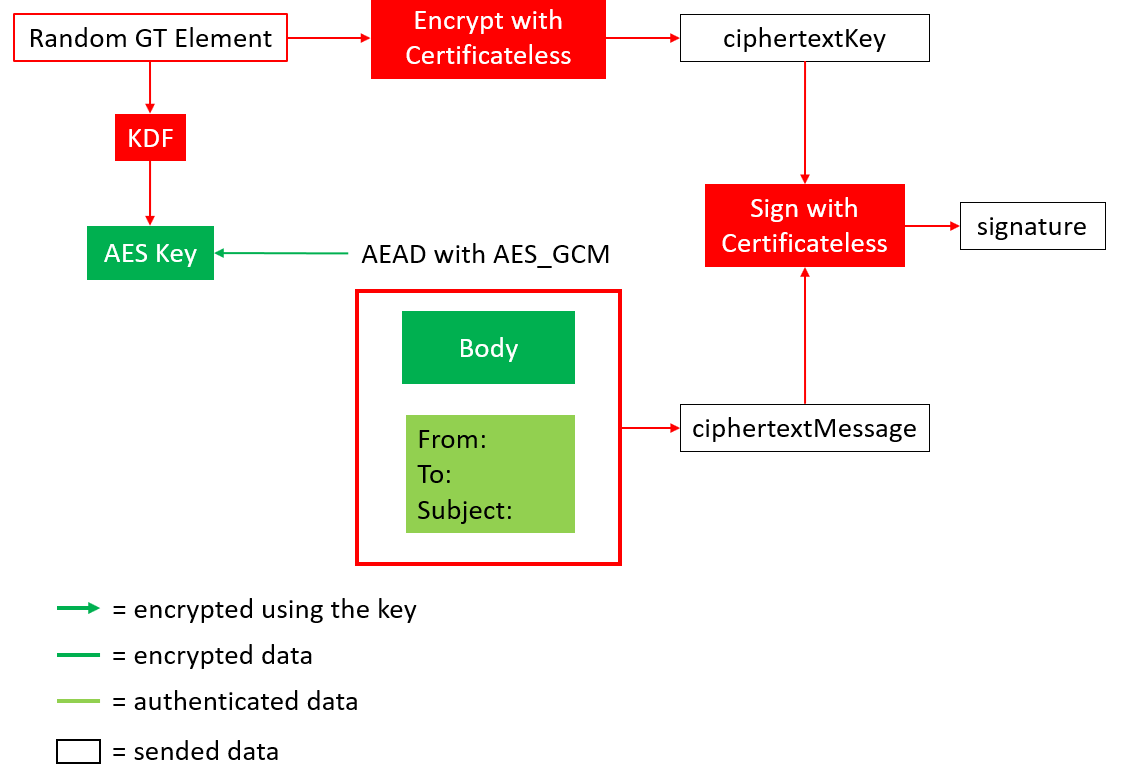
\includegraphics[width=\textwidth]{images/schemCles.png}
	\caption{Schéma encapsulation des données}
	\label{fig:encapsulate}
\end{figure}

\section{Fonctionnement global POC (KGC)}
Présentation du fonctionnement global de l'implémentation du KGC pour le POC. De plus, les problèmes connus et des propositions d'améliorations sont présentés.
\subsection{Fonctionnement}
Le KGC est un élément important du protocole, en effet c'est lui qui va fournir une partie de la clé privée de l'utilisateur. Dans ce cas, il permet de distribuer les clés publiques de ses utilisateurs, mais habituellement on fera plutôt appel à un serveur dédié pour la gestion des clés.

Par mesure de généricité j'ai établi des codes d'opérations (arbitraires) afin de définir les opérations demandées au serveur par le client. Cela à l'aide de la librairie binn et les constructions d'objets proposés.

\paragraph*{Structure des paquets reçus.}
Pour la structure des paquets que le KGC va traiter, ils se présentent sous la forme d'un objet binn qui a comme propriétés au moins un code d'opération \textbf{opCode} et un \textbf{ID} associé. Cela permet de trier le paquet et de l'associer à une opération afin de traiter la donnée amenée avec le paquet. L'ID sert aussi différemment en fonction des codes employés.

Ainsi un paquet typique sera :\\
\{opCode: PK, ID : alice@wonderland.com, payload : xxx\}
\paragraph*{Codes d'opérations.}
Les différents codes d'opérations sont :
\begin{itemize}
	\item HELO : Permet de s'annoncer au KGC pour la première fois, le KGC répondra systématiquement avec les paramètres globaux du système. Cela implique la Master Public Key de chiffrement du KGC ainsi que celle du schéma de signature. 
	\item PK : Permet d'annoncer les clés publiques de l'utilisateur avec un certain ID. Le paquet est composé de \{ID : alice@wonderland.com, opCode : PK, PKE : base64 de la PKE, PKS : base64 de la PKS\}. La PKE est encodée en base64 par le client puis est envoyée au serveur. Elle est aussi représentée à l'aide d'un objet binn mais le serveur n'a pas besoin d'en prendre connaissance, il stocke donc cette donnée telle quelle dans la base de donnée NoSQL. La même chose est faite pour la PKS, la clé publique pour la signature.
	\item GPE : Permet de récupérer la clé publique de chiffrement (utile pour chiffrer un message) d'un utilisateur ayant l'ID mentionné. Ainsi le serveur va simplement regarder dans la base de donnée pour "encryption/ID" et récupérer la clé encodée en base64 et la renvoyer à l'utilisateur. Si le serveur ne trouve pas cette clé, il va renvoyer une erreur dans l'objet et ainsi à la réception on va d'abord regarder cette erreur.
	\item GPS : Fonctionne de la même manière que "GPE" mais pour les clés publiques de Signature (utile pour vérifier une signature).
	\item SE : Permet de faire la "Signature Extraction" et donc de demander la Partial Private Key pour l'utilisateur ID. Utilisé lors de la signature d'un message afin de construire sa clé privée et de signer le message avec. 
	\item EE : Permet de faire la "Encryption Extraction" et donc de demander la Partial Private Key pour l'utilisateur ID. Utilisé lors du déchiffrement d'un message pour reconstruire sa clé privée.
\end{itemize}
\subsection{Problème rencontré}
Un problème ayant bien ralenti le développement est une erreur dans l'implémentation des socket en C. En effet, au départ le serveur ne recevait pas toutes les données du client et inversement d'ailleurs.

La solution a été de recevoir les données par petits chunks et de les regrouper petit à petit. Beaucoup de tests et de recherches ont été faites pour ce problème pourtant anodin sur les socket en C.
\subsection{Problèmes connus}
Liste des problèmes connus concernant l'implémentation du côté serveur.
\paragraph*{Implémentations TLS}
Pour avoir une sécurité supplémentaire et garantir l'authenticité des paramètres envoyés par le KGC il serait préférable d'implémenter les serveur en TLS. Ceci n'a pas été fait dans l'état actuel du projet.
\paragraph*{Sauvegarde des paramètres}
La sauvegarde des paramètres privés du serveur n'est pas implémentée dans le KGC actuellement ce qui amènerait des problèmes lors d'un crash ou un arrêt du serveur. Ceci doit être résolu dans une implémentation effective.
\paragraph*{Révocation des clés}
La révocation des clés n'est pas réellement implémentée, dans l'état actuel le serveur va reprendre une nouvelle clé publique envoyée d'Alice car aucune vérification n'est faite, ceci permet de révoquer une clé en l'écrasant. Cependant ce n'est pas une vrai révocation de clés.
\subsection{Améliorations}
Quelques améliorations seraient possibles mais restent à mettre en place, cela permet de donner quelques pistes pour la continuation du travail :
\paragraph*{Vérification email.}
Implémentation d'une vérification par email afin d'être sûr que l'adresse email annoncée appartient bien à l'utilisateur qui s'authentifie pour la première fois. Typiquement lors du "HELO", on pourrait envoyer un mail de vérification avec un code sur l'email annoncé (s'il n'est pas dans la base de données) et demander le code envoyé avant de pouvoir uploader sa clé publique. Ainsi le client devrait pouvoir implémenter cette fonctionnalité aussi. Cela permettrait d'être sûr que tel utilisateur a effectivement tel email.
\paragraph*{Mise en place à large échelle}
Si l'on veut pouvoir mettre en place ce genre de système à une large échelle, il faut prévoir une manière d'avoir plusieurs KGC qui communiquent, par exemple, entres eux dans un système global de réplication. Ceci afin de pouvoir avoir les mêmes paramètres sur l'ensemble des KGC et que le système fonctionne.

Une autre solution serait par exemple d'ajouter un "tag" d'appartenance à un ID et celui-ci sera donc lié à un certain KGC. Ceci afin de partager la charge qui serait normalement sur un seul KGC. Ce genre de solutions pourrait permettre d'avoir par exemple un KGC par domaine ou alors de les partager via les TLDs. De plus, les KGC pourraient avoir des paramètres générés différemment entre eux, ce qui ne serait pas le cas dans un système de réplication. Cette solution ajoute cependant de la complexité au système. Et des envoi de paquets plus volumineux sur le réseau pour les paramètres globaux d'un KGC qui sont de 52kB, pour chaque KGC.

Pour le système de clés on pourrait reprendre l'idée de~\cite{journals/ijnsec/BalakrishnanR16} afin d'aller chercher le serveur de clés pour tel domaine.
\section{Fonctionnement global POC (Client)}
Présentation du fonctionnement global de l'implémentation du client mail implémentant la CLPKC pour le POC, des améliorations possibles et des problèmes connus.
\subsection{Fonctionnement}
Le déroulement pour envoyer un message se passe comme suit :
\begin{itemize}
	\item Informations de connexions à GMail demandées
	\item Si le fichier (\textit{globalMPK}) de paramètres globaux n'est pas présent en local l'application communiquera avec le KGC afin de récupérer ces paramètres publiques tels que $mpk_E$ et $mpk_S$ et les stockera donc.
	\item Si le fichier (\textit{ID\_SK}) n'est pas trouvé les valeurs secrètes vont être tirées pour l'utilisateur et la construction des clés publiques et leur envoi au serveur va être effectué. Si le fichier est trouvé il va être déchiffrer en utilisant AES\_GCM en prenant la clé donnée par l'application de l'algorithme Argon2id sur un mot de passe donné par l'utilisateur.
	\item L'application va demander si l'utilisateur veut envoyer ou recevoir des emails.
	\item Dans le cadre d'un envoi, les informations nécessaires à l'envoi d'un mail seront demandées telles que le destinataire, le sujet et le message.
	\item L'application va regarder si le fichier \textit{ID\_PK} est disponible en local et si ce n'est pas le cas il va demander au KGC la clé publique du destinataire. Si le KGC n'arrives pas à la trouver une erreur sera annoncée à l'utilisateur et l'envoi ne sera pas effectué.
	\item Si tout est bon l'application va effectuer l'encapsulation des données montrées dans la Figure \ref{fig:encapsulate}.
	\item L'envoi est effectué via SMTP en incluant dans les headers le base64 des informations nécessaires à la réception.
	\item Les informations confidentielles sont sauvegardées en les chiffrant à l'aide AES\_GCM et Argon2id afin de dériver le mot de passe de l'utilisateur.
\end{itemize}
La réception se passe de la même manière globalement, le changement principal et le téléchargement des emails des dernières 24h grâce à IMAP, à moins qu'ils soient déjà téléchargés auparavant. Le déchiffrement va se passer comme décrit dans le Chapitre \ref{ch:arch}. 
\subsection{Fonctionnalités}
\paragraph*{Sécurité connexion mail.}
Pour la connexion au serveur SMTP / IMAP j'ai fait attention à la connexion sécurisée pour éviter de \textit{leak} des mots de passe des utilisateurs du POC. En effet, cela permet de chiffrer les communications avec les serveurs de Gmail comme démontré dans la Figure \ref{fig:securityProofEmail}.
\begin{figure}[h!]
	\centering
	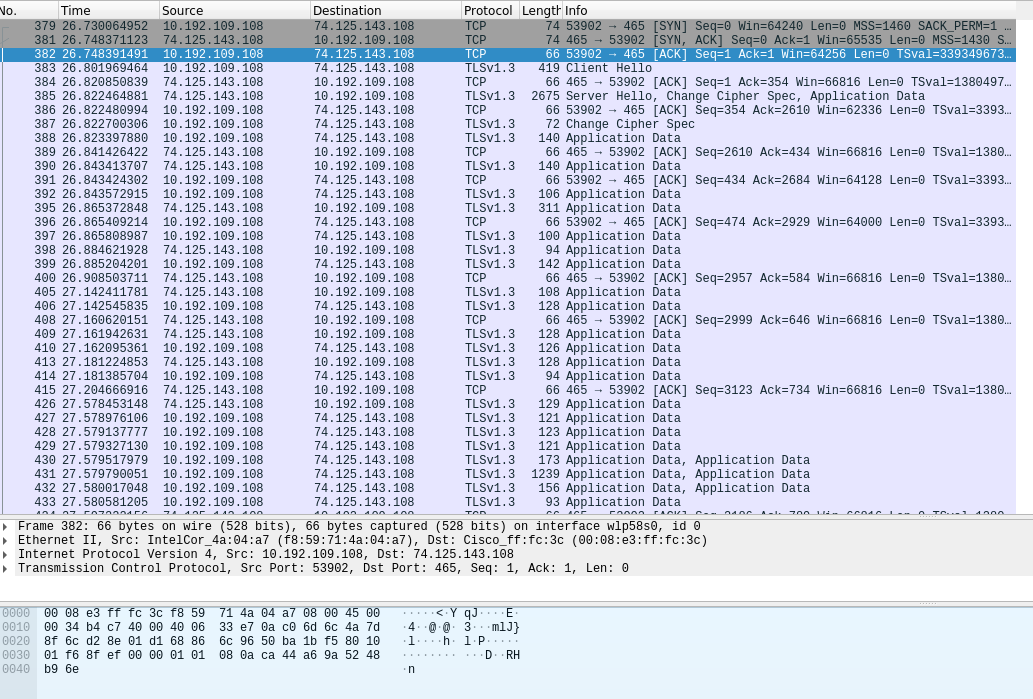
\includegraphics[width=14cm]{images/packetProofEncrypted.png}
	\caption{Connexion SSL/TLS avec le serveur email}
	\label{fig:securityProofEmail}
\end{figure}
\subsection{Problèmes connus}
Les problèmes qu'il reste à résoudre à ce jour :
\paragraph*{Développement sécurisé.}
Lors du développement j'ai fait attention au maximum d'avoir le moins possible de fuites mémoires à l'aide de sanitizers et de valgrind. Cependant cela ne suffirait pas pour une application correctement sécurisée, il faudrait mettre à 0 les structures utilisées et qui stockent des informations confidentielles.
\paragraph*{Enregistrement lors d'un crash}
Lors d'un crash du client en plein milieu du programme ou de l'écriture/chiffrement du fichier des secrets il se peut que celui-ci deviennent corrompu. Il faudrait éviter de le corrompre car la seule manière d'y remédier serait de le supprimer et ainsi de recréer ses valeurs secrètes.
\subsection{Améliorations}
Les améliorations à amener dans le client :
\paragraph*{Multiples destinataires.}
Pour le moment l'implémentation ne prends pas en compte une situation où un mail doit être envoyé à des destinataires multiples, c'est une fonctionnalité importante à mettre en œuvre dans une implémentation de client mail. Pour ce faire, il faudra spécifier dans les headers l'utilisateur ciblé par tel cipher et signature. Ainsi, lors de la réception, le client prendra les options X-ID-CIPHER-B64 p.ex. Ou alors trouver un moyen d'envoyer un mail différent à chaque utilisateur, sans perdre la possibilité qu'un destinataire puisse choisir de répondre à tous les autres destinataires.
\paragraph*{Possibilité d'ajouter des pièces jointes.}
Pour le moment la possibilité d'ajout de pièces jointes n'a pas été pris en considération. Cependant, une des librairies choisies pour la réception des mails pourrait composer des messages contenant des pièces jointes. Il faudrait ainsi les chiffrer avec la clé symétrique avant de l'ajouter dans le mail.
\paragraph*{GUI.}
Mettre en place une interface utilisateur pour le client mail, cela aiderait à rendre le chiffrement plus transparent et plus simple pour l'utilisateur. En effet, demander à l'utilisateur d'écrire son mail au terminal n'est pas spécialement agréable.
\paragraph*{Ajout clé publique}
Dans l'envoi du mail il faudrait ajouter la clé publique de la source dans le message, ainsi que la vérification de la signature.

\paragraph*{Répudiation et non répudiation}
Ajouter la possibilité de signer ou non l'email afin de pouvoir obtenir ou non de la répudiation. Pour le moment l'implémentation signe le message et la clé symétrique chiffrée, ainsi la non-répudiation est accomplie. Afin d'avoir de la non répudiation il faudrait ne plus avoir cette signature, cela permettrait d'avoir la répudiation et d'avoir tout de même un système sécurisé.

\section{Comparaisons avec l'état de l'art}
Dans cette section je vais présenter les différents protocoles et implémentations existantes présentées au Chapitre \ref{ch:analysis} et les comparer à l'implémentation faite dans ce travail (ci-après CLPKC-POC). Tout d'abord en présentant les différentes propriétés cryptographiques, les tailles d'overhead et l'utilisabilité.

\subsection{Propriétés cryptographiques}
Ici je fais un comparatif sur les différentes propriétés cryptographiques que les systèmes de mails sécurisés proposent avec mon implémentation Certificateless. On peut le voir dans la table \ref{table:comparisonProperties}. La pseudo forward secrecy est intéressante mais expliquée dans la Section \ref{subsec:pseudoSecrecy}. La répudiation est une propriété possible dans CLPKC en évitant de signer la clé symétrique chiffrée. La non répudiation est établie via les signatures digitales des différents algorithmes, dans CLPKC POC la signature se fait sur le message chiffré et la clé chiffrée ainsi la source ne pourra répudier le fait d'avoir signer ces données. 
\begin{table}[h!]
	\centering
	\begin{tabular}{ |p{3cm}||p{3cm}|p{3cm}|p{3cm}| }
		\hline
		\multicolumn{4}{|c|}{Comparaisons des propriétés cryptographiques proposées} \\
		\hline
		Propriétés & CL-PKC POC & PGP & S/MIME \\
		\hline
		E2EE   & Oui & Oui & Oui\\
		Forward Secrecy & Oui (Pseudo) & Non & Non\\
		Repudiation & Possible & Non & Non\\
		Non repudiation & Oui & Oui & Oui\\
		\hline
	\end{tabular}
	\caption{Table de comparaison des différentes propriétés cryptographiques }
	\label{table:comparisonProperties}
\end{table}
\subsection{Overhead induit}
Ici je présente les différents \textit{overhead} que j'ai remarqué en utilisant les différents systèmes de mails sécurisés analysés au Chapitre \ref{ch:analysis}. Dans le tableau \ref{table:comparisonOverhead} on voit la taille d'overhead induit par les différents systèmes testés. Ces tailles ont été déterminées de manière empirique par des tests effectués tout au long de ce projet.
\begin{table}[h!]
	\centering
	\begin{tabular}{ |p{3cm}||p{4cm}|p{6cm}| }
		\hline
		\multicolumn{3}{|c|}{Comparaisons de l'overhead induit dans un mail} \\
		\hline
		Implémentations & Taille overhead & Contenu\\
		\hline
		CLPKC-POC   & Environ 1000 bytes / destinataire & Signature, timestamp, nonce, Encrypted Session Key\\
		PGP & Environ 300 bytes / destinataire & Encrypted Session key\\
		S/MIME & Environ 7300 bytes (Signature) & CMS EnvelopedData et Certificat\\
		\hline
	\end{tabular}
	\caption{Table de comparaison des différents overhead en rapport avec les solutions existantes }
	\label{table:comparisonOverhead}
\end{table}

\subsection{Différences d'utilisabilité}
Comparaison de la facilité d'utilisation entre PGP, S/MIME et CLPKC-POC. Cela permet de comparer les différents cas d'utilisation et de voir la souplesse des différentes solutions.

\paragraph*{Usage global}
Globalement l'utilisation de CLPKC-POC est souvent plus simple que l'utilisation de PGP ou S/MIME. En fait, l'utilisation sera plus simple car le système de cryptographie \textit{Certificateless} a certaines propriétés qui le rend plus accessible. 

Dans S/MIME le contrôle des certificats et l'import de différents certificats est complexe et peut entrainer des erreurs. Dans PGP les clés ne sont pas si faciles à obtenir et les clés nécessitent aussi d'avoir une certaine confiance (signés par d'autres utilisateurs) de PGP.
\paragraph*{KGC / serveurs de clés non accessibles}
Que se passe-t-il si un serveur de clés ou le KGC n'est plus accessible pour une quelconque raison ?

Dans le cas de PGP, le déchiffrement pourra être effectué car la clé privée ne change pas d'un moment à l'autre. De plus, lors d'un chiffrement PGP la signature digitale est effectuée sur le texte clair puis est chiffrée avec. Ainsi la clé publique de la source doit être récupérée, cela posera un problème si la clé n'est pas déjà stockée en local. Dans certains cas la clé publique peut être intégrée à l'envoi dans l'email mais n'est pas authentifiée.

Dans le cas de CLPKC-POC, le déchiffrement sera potentiellement compromis, cela dépendra si l'utilisateur aura créé la clé pour la semaine courante ou non. Si c'est le cas, le chiffrement pourra être fait. La vérification de la signature pourra être faite aussi si la clé publique de la source est stockée en local (si l'utilisateur nous a envoyé un mail auparavant). Il serait possible d'envoyer la clé publique de la source pour faciliter la vérification mais ce n'est pas fait dans l'état actuel.

Dans S/MIME, le déchiffrement pourra être effectué car la clé privée ne changera pas non plus. La vérification pourra être faite en local avec les CAs intégrés dans le système pour le certificat envoyé avec le mail.
\paragraph*{Erreur utilisateur}
Les erreurs que les utilisateurs peuvent faire sur certains éléments peuvent être problématiques dans certains cas pour PGP et S/MIME. En effet, si un utilisateur signe une clé publique d'un utilisateur sans vérifier réellement l'identité cela pourrait authentifier une clé publique compromise et déstabiliserait le \textit{Web Of Trust}.

 Pareil pour S/MIME où l'import d'un certificat malicieux pourrait avoir un impact sur la sécurité des données. Cependant, dans CLPKC-POC peu d'erreurs peuvent être faites car la plupart des paramètres et clés sont générés automatiquement.